% !TeX encoding=utf8
% !TeX spellcheck = en-US

\section{Introduction}
\label{sec:intro}

Information and Communication Technologies (ICT) are being adopted as a catalyst in the smart city domain, on top of which novel services are developed and legacy ones are evolved. In addition, the pervasive presence of ICT allows service providers and stakeholders to directly interact with citizens to continuously improve services in a co-creative manner. This co-creation approach permits the rapid deployment and adoption of innovative solutions for urban challenges~\cite{nasrawi}. A central part of instrumenting a smart-city with an IoT infrastructure is to be able to sense and monitor how the city performs, and to understand the dynamics of the city as a system. As examples, it becomes possible to examine how people make use of urban environments, and parameters like pollution, can be visualized and tracked throughout the city.

Recently, co-creation has been exploited in different ways by various \textit{Experimentation-as-a-Service} (EaaS) frameworks~\cite{vermesan2015building}. By ``co-creation'', we refer to the process of involving citizens and other stakeholders in designing as well as developing smart city solutions, and using local know-how to respond to existing challenges in modern cities and their communities.
For instance, Pallot and Pawar investigate co-creation to improve QoS~\cite{pallot}, while gamification techniques are used by Pokrić et al.~\cite{pokric}. Participation and interaction with stakeholders are used to attract people to the co-creation process~\cite{phuluwa, celino, gozard}. Finally, other work, such as Schaffers et al. ~\cite{schaffers2011}, focuses on technical aspects, in particular IoT or machine-to-machine communications, leaving aside user/citizen interaction.  In this sense, the scope of existing EaaS frameworks is limited to specific services or challenges. However, we believe that end-to-end solutions are necessary for harnessing the potential of complex city ecosystems. At the same time, the diversity in potential smart city applications makes it hard for a monolithic solution to satisfy their varied requirements. 

\begin{figure}
	\centering
	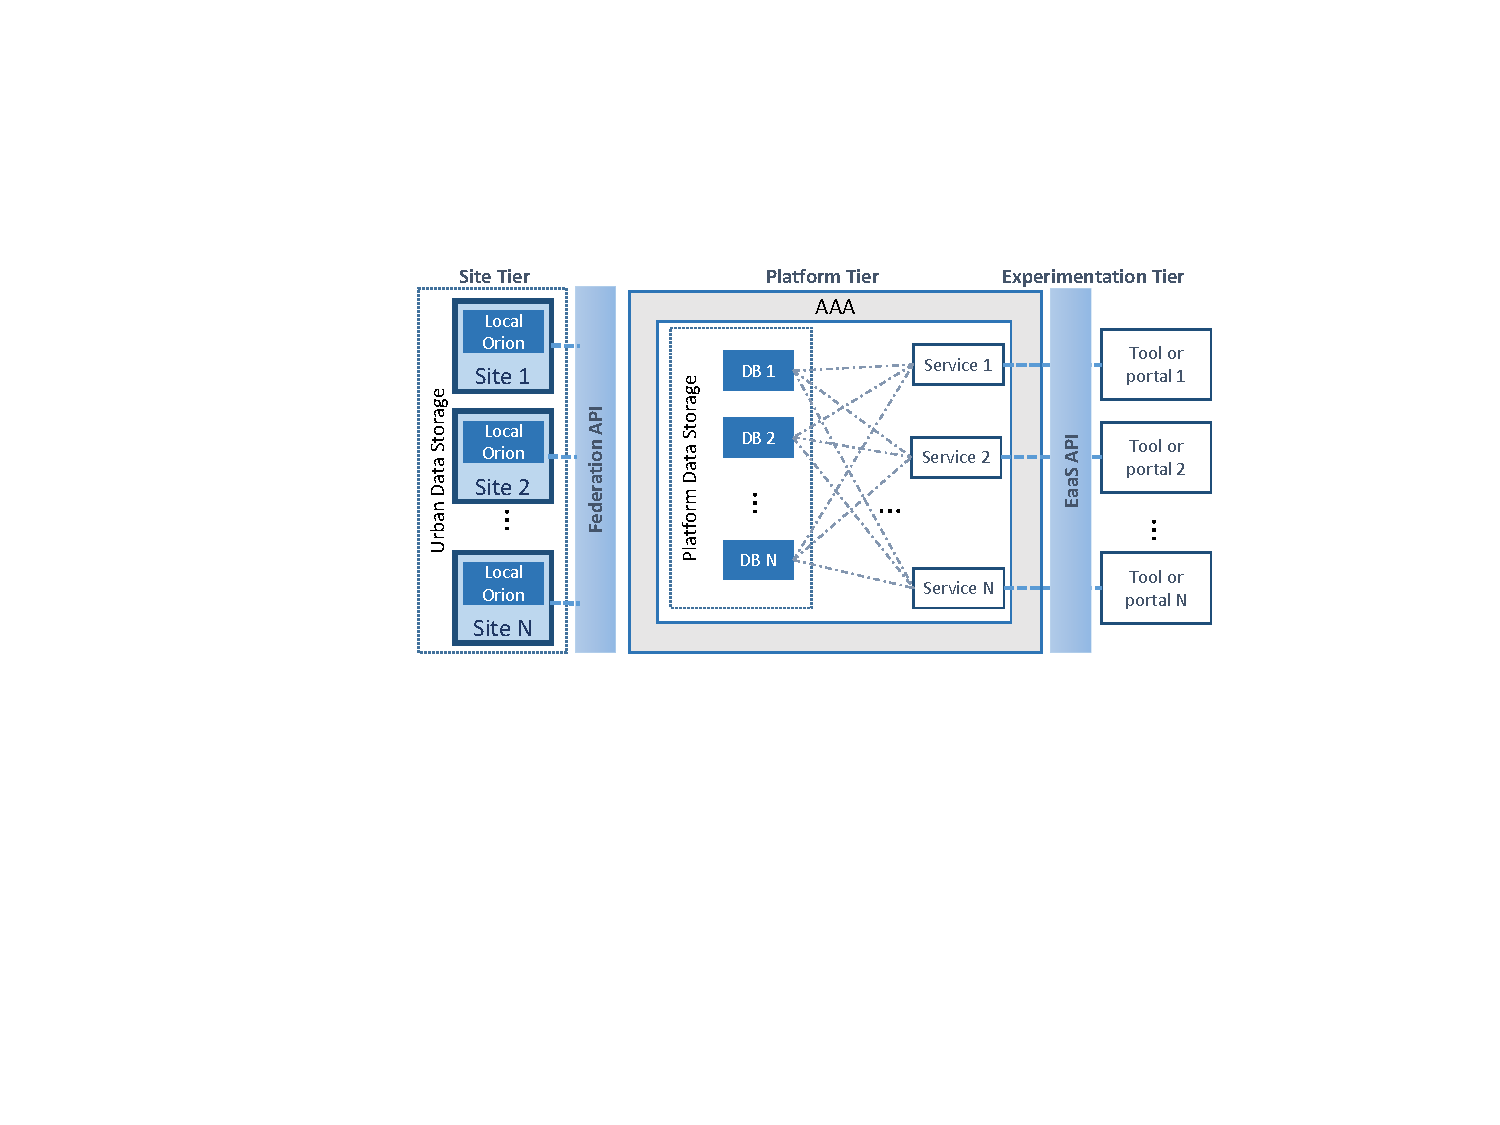
\includegraphics[scale = .66]{figures/simpleArchH}
	\caption{Overall OrganiCity platform architecture}
	\label{fig:arch}	
\end{figure}

In this context, the OrganiCity\footnote{OrganiCity H2020 project, http://organicity.eu} EU project (OC) developed a customizable EaaS framework, called the \emph{OC platform}. \highlighttext{The OC platform provides a common playground where different stakeholders can co-create urban services~\cite{gutierrez1}, and adopt the functionalities offered by the platform that better serve their needs}. As depicted in \Cref{fig:arch}, its design follows a three-tier approach~\cite{Schuldt2009}, addressing data provisioning, platform management, and experimentation support. It has been developed following an experimentally-driven approach, supported by \emph{open calls} during two periods (first open call in 2016--2017 and second open call in 2017--2018). \highlighttext{Open calls have had a twofold objective: first to help maturing the platform by gathering feedback from external users; and secondly to analyze the platform sustainability for the future.} \highlighttext{Throughout this paper, accepted open call projects are termed \emph{experiments}, and the actual people conducting these are referred to as \emph{experimenters} and \emph{experiment team} interchangeably. In addition, the term \emph{experimentation} refers to the process of conducting an actual experiment.}

\highlighttext{The first version of the OC platform~\cite{gutierrez1} was designed and validated within the OrganiCity consortium. This initial version was exploited during the first open call, which served to gather information and feedback from experimenters. Afterwards, the platform was tweaked according to the feedback and the new version was released in the second open call, which was devoted to developing a co-creation methodology for establishing cross-collaboration between stakeholders, communities, sectors and countries in a smart city context. In this paper we focus on the technical evolution, so that the work presented hereinafter spans from the period from which the OC platform was first deployed (initiation of first open call) to shortly before the second open call. In the first open call, a number of experiments have been selected and implemented, over a period of six months. Thanks to this key part of the OC project, experimenters have played an active role in the design and validation of our platform.}

In the following, we present a toolset to foster the development of urban services in a co-creative way. These novel services have been identified based on the feedback provided by 25 experiments conducted in five European cities (being from United Kingdom, Denmark, Spain, Greece, and Belgium), which have resulted in creating pilot services for more than 10 different urban application areas. In addition, the experiment teams involved different types of stakeholders, ranging from individual citizens to Small and Medium-sized Enterprises (SMEs), or public authorities. To our best knowledge, this is the first time that an EaaS framework is adopted in such a large scale manner, spanning over multiple cities. 

The rest of this work is structured as follows. First, \Cref{sec:sota} provides a discussion of related work, highlighting differences between existing approaches and ours. \highlighttext{Then, In \Cref{sec:lear}, the most relevant feedback obtained during OC platform exploitation, as well as possible modifications are explained. In \Cref{sec:adv} we describe the services developed after the first experimentation period, highlighting their functionalities and benefits.}  Finally, \Cref{sec:con} concludes the paper.